\documentclass[10pt,twocolumn,letterpaper]{article}

\usepackage{fullpage}
\usepackage{graphicx}

\author{David Simon}
\title{Task-Specific Filesystem Block Reorganization in Ext3}

\begin{document}

\maketitle

\begin{abstract}
Hard disk access times are the most significant performance bottleneck when
starting typical applications on contemporary personal computers and servers.
Most modern programs must load numerous libraries, resource files, modules, and
other pieces of information off disk before performing any useful work. Optimization
in this area should prove fruitful.

We attempted to reduce the amount of time consumed by hard disk activity during
the initialization of various programs. To do this, we observed which data blocks were
used during the initialization of various programs. Then, those blocks were moved
closer together, in the hope that the quantity and length of drive head seeks
would be reduced. The results were mixed; some applications received no particular
benefit from this optimiziation, while others were made to start significantly faster.
\end{abstract}

\section{Introduction}

Hard disk drives are, by a wide margin, the slowest internal storage devices commonly
used in modern computing. For a typical read or write, the disk head must first
\emph{seek} to the target block\cite{seektime}. On even the fastest hard disks\cite{deskstar}, one seek
can take several milliseconds, often orders of magnitude longer than the operation which will actually
use that data. Even if seeking is unnecessary because the disk head is already at the correct track, there is
often still a long delay waiting for the desired block to spin around to the head again\cite{latency}. When
many disk operations are required, tasks that would otherwise be immediately performing computations on data must first wait for these slow, mechanical processes to complete.

Ideally, to mitigate this problem, the next block to be requested should be physically near to
and after the current block\cite{autolocality}. When a seek or
spin wait is unavoidable, then it is better if the travel time required can at least be lessened by reducing the
physical distance between the current block and the next. The best scenario is when
as much disk time as possible is spent actually retreiving data, and as little as possible
wasted travelling from one request location to another.

It should be possible, with intelligent organization of data on the disk, to make the hard drive behave
more closely to this ideal. Bolero, the Block Organizer that Localizes Empirically-Related Objects, was developed as a proof-of-concept for this idea.

\section{Motivation for Bolero}\label{sec:motive}

In most filesystems, files are divided up
into one or more fixed-size chunks, called \texttt{blocks}CITETHIS. When a file's blocks
are not contiguous on disk, then the file is \texttt{fragmented}
and operations that require more than one block from the file are slow due to
seek and spin delays. The best proactive way to prevent fragmentation is to find contiguous
chunks of available space when allocating new files. Some older filesystems, such as FAT, were
very ineffective at doing this\cite{fathistory}.
FAT filesystems frequently had to be \texttt{defragmented} to maintain performance.
Modern filesystems, such as NTFS CITETHIS and ext3 CITETHIS, keep better track of free space,
and do not tend to fragment until the filesystem becomes nearly full. Advanced filesystems sometimes
use even more sophisticated strategies to prevent fragmentation, such as preallocating extra room to allow 
contiguous appending, or delaying physical allocation as long as possible so that better guesses
can be made about the characteristics of newly created files\cite{xfs}.

As important as these advancements have been, however, they do not address another, more subtle form of fragmentation: fragmentation between related files.
Just as slowdowns result when the various blocks of a file are distant from each other, when \emph{files} accessed in sequence are far from each other on the disk, significant unnecessary delays may result. For example, a large application such as an office suite or desktop environment requires numerous programs, shared libraries, icons, fonts, and other resources before it can start up completely. If these files must be read from disk but are spread apart from each other, the application's startup time will increase.

The objective of Bolero is to reduce this type of fragmentation for that specific case, that of applications
starting up and loading a variety of resources from disk. It accomplishes this by moving data blocks that are typically accessed at about the same time closer together, and re-sequencing them into the order they are expected to be accessed. There are two possible strategies to accomplish this : general optimization and task-specific optimization.

With general optimization, the reorganizer would use the recorded observations
to determine which files tend to be accessed within a short time from each
other, and in what order. It would then place files on disk in such a way as
to reduce average seek time and spin latency throughout the computer's operation.
Previous attempts at implementing this type of optimization at a
sub-filesystem level have resulted in significant performance benefits\cite{autolocality}.

The other approach, task-specific optimization, is simpler to
implement and may also (for its specific purpose) result in better performance. With this
approach, observations are limited to a particular, short-term task. For example,
the objective may simply be to get the computer's desktop environment to load
quicker after a cold boot. Within a short but disk-intensive period like this, even
though there will have been a lot of disk activity, any single file will
probably have been read from disk only once. The reorganizer can therefore simply
rearrange the relevant files on the disk to be contiguous and in the same order as that
recorded during the observational period, to reduce the amount of time taken for
that particular task. Previous efforts using this approach have been
successful in reducing large application startup times by over 60\%\cite{ala}.

Because task-specific optimiziation is easier to implement and readily suggests
a metric, we chose it as the approach used by Bolero. However, since that approach is a
specialization of the general optimiziation approach, its success may be seen
as a motivation to explore the more complex, but potentially more rewarding, area
of general optimiziation.

For this project, we attempted to improve the startup time of the following applications with this approach:
\begin{itemize}
\item X Windows + KDE
\item OpenOffice
\item MySQL
\end{itemize}
Among these three applications, a wide range of shared libraries, subsystems, and user interface types
are involved. This helps to eliminate the influence of these factors on the final results;
ideally, the only factor being tested should be disk usage.

The test environment was a default installation of Kubuntu 8.04 on a 12GB partition located
at the end of the 61.4GB test hard disk, a PATA Maxtor 6Y060L0. The test system had
1GB of RAM, and a 2.4Ghz processor. This combination of a somewhat powerful system and
a somewhat meidocre hard drive was chosen purposefully: this scenario exacerbates the
problem of the hard drive as the bottleneck of the application loading process, and therefore
any improvement due to the optimization process should be especially noticable.

\section{Filesystem Manipulation}

Because of the relative ease of extending and manipulating Linux filesystems and
kernel code, Bolero was be developed targetting Linux environments with ext3
filesystems. Ext3 is the standard filesystem used in Linux
environments, and is largely backwards compatible with ext2\cite{ext2journal}.
The general approach used by Bolero, however, is also applicable to most other commonly-used
filesystems.

The basic mechanism used by Bolero is the \texttt{libext2fs} library. This C
library, part of the standard \texttt{e2fstools} package, allows user-space programs
to open, scan, and make changes to ext2 filesystems. For Bolero, we wrote
a Python wrapper called \texttt{pyext2} around a subset of this library's functionality.
This library can open and scan through an ext2 or ext3 filesystem, report
various information about its contents, and swap the locations of arbitrary data
blocks while maintaining the filesystem's internal consistency.

Although there are some tentative mechanisms to allow the online rearrangement
of ext3 blocks\cite{ext3online}, Bolero is designed to run only on unmounted filesystems.
While it would be
convenient for the user to be able to manipulate a mounted filesystem, doing so
would add unnecessary complexity, making debugging and
development more difficult than necessary. Working with unmounted filesystems,
the reorganizer code can stay entirely in user-space, and does not have
to deal with the possibility of the file system's state being changed
midway through the process by other mechanisms outside its control.

With only the basic tool of swapping data blocks, a wide range of possible
defragmentation techniques are possible. Bolero includes \texttt{defragment.py}
a very simplistic, traditional defragmenter for ext3, which
does nothing but reduce fragmentation within individual files. Because ext3 files do
not usually tend to fragment, the case for this kind of reorganization alone
is not very strong. However, individual file defragmentation is an important
basis for later, more sophisticated operations, and also serves as a useful test
of the system's ability to safely and correctly alter filesystems.

Once the reorganizer can reduce file discontiguity, it is possible to
use that same mechanism to reduce inter-file discontiguity, as explaiend
in section \ref{sec:motive}. Both types of defragmentation are necessary because the overall goal is to reduce the quantity of seeks and spin waits. The ideal state of affairs is for the disk to travel through
a sequence of files without interruption\cite{autolocality}, from the first block of the first file to the last
block of the last file with no delays or seeks.

This ideal is difficult to acheive completely, due to the realities of hard disk
and filesystem layout. For example, in ext3, data blocks are organized into larger
collections on disk called \texttt{block groups}\cite{ext2intro}. Each
block group contains actual data blocks as well as other information, such
as bitmaps describing available space, and tables of \texttt{inodes},
which describe meta-data for each file. These areas of meta-information within
groups create ``gaps'' of disk area which the defragmenter cannot
use to reduce discontiguity, because there can never be file data there.
The current implementation of Bolero ignores this problem and simply
skips over these gaps. A more subtle defragmenter might attempt to arrange
files around these gaps in anticipation of access patterns.

There are many other issues which present similar complications to a defragmentation
system, such as track boundaries, unusual varities of file data (i.e. directories, which
are almost never scanned through linearly), and files which are expected to change
size or be deleted during normal operations. The Bolero defragmenter makes no attempt to
solve even these relatively common complications.

However, even an unsubtle implementation such as Bolero can serve as a proof-of-concept
to demonstrate the validity of the basic idea. If a repeatable, signifiacnt improvement
is observed after making simplistic improvements to the filesystem layout, it follows
that more sophisticated improvements should yield even better results.

\section{Observing Disk Activity}\label{sec:observing}

The major difference between the Bolero defragmenter and a traditional defragmenter
is that information about the relationships between files (specifically, the order
in which tend to be are accessed during specific tasks) is used. We developed a few
simple observation tools to record such information. These same tools were also used to record
timing information for each of the target tasks, in order to determine how much improvement
the optimization process was yielding, as described in section \ref{sec:results}.

For each task in each state (either the untouched control state or an optimized state), the
following procedure was used to collect observational data:
\begin{enumerate}
\item A \texttt{proc}-based mechanism is used to clear the Linux system's software-based disk cache. CITETHIS
\item Thirty MB is read from the beginning of the target drive, far from the target filesystem, in order to deceive the drive's internal cache. Without this step, test results tended to change as subsequent tests were performed, as the drive restored information from its cache rather than seeking to and reading the physical data itself.
\item If applicable, a tool called \texttt{frecord} is started, which would monitor for new processes starting up and record which
files they opened.
\item A timestamp is taken, and the target program is started.
\item When the program is finished loading (the definition of which is dependent upon the particular program being observed), the elapsed time is recorded, and \texttt{frecord} is stopped if it had been started earlier. It is at this
point that \texttt{frecord} writes its collected information to disk.
\item The target program is killed.
\end{enumerate}

For each target program, this procedure was repeated 100 times. For each run of the procedure, the \texttt{frecord}
process noted which processes started up after its initialization. Every 3 milliseconds, the open files of each
of these processes were recorded to memory. Afterwords, the information in these 100 recordings of file usage
was collected by the \texttt{fsummarize} tool, which uses it to produce a best-guess list of all the files
that might be opened the next time the target application starts up, in the order they are most likely to be
opened in. All files which were opened in even one of the recorded sessions are included in the list. n theory,
it is better to include an unnecessary file and have the disk head skip over it with relatively little expense than to omit it and force the disk to (even occassionally) perform an expensive seek to some other part of the disk
and then back.

\section{Defragmentation}

There are two defragmenters included with Bolero that can make use of the results from \texttt{fsummarize}:
\texttt{defragment.py} and \texttt{mdefragment.py}. The former locates every data block for every file mentioned
in the summary, and puts them in sequential order on disk, starting at the first block of the group containing
the first inode. The latter, \texttt{mdefragment.py}, acts in a similar way, but instead starts at the group containing the mean from all inodes involved. This was done as an attempt to reduce the average seek distance for
those remaining seeks which must be performed, particularly seeks to inode table entries (see section \ref{sec:future}).

After defragmentation, the blocks that were originally in the area that the task-related blocks were sorted to
are strewn arbitrarily around the disk. This is acceptable for the purposes of this project, since those (now
discontiguous) files are unlikely to be accessed during the target task at all; if the target application being observed loads the same functionality every time it is started, and a file hasn't been noticed
in even one of the 100 \texttt{frecord} observational runs on that application, then it's a safe assumption that that file is not related to the application's loading process. However, the file may still be need for some other application or task. For that reason, a Bolero-like approach applied to a production system would have to be more considerate of those data blocks it must move out of the way.

\section{Measuring Results}\label{sec:results}

In order to gauge how successful any optimization is, it is important to have
repeatable, objective measurements. For the specific task that Bolero was written
to address, optimizing the startup time of various applications, this means that it
is necessary to have a way to accurately measure the amount of time it takes for
a program to startup, and then to perform that measurement a statistically significant
number of times on both a control filesystem and a filesystem optimized for that program.

However, this measurement is more ambiguous than we initially expected, and a few
somewhat arbitrary choices had to be made. The most important of these is the problem of determing when, exactly,
a program has ``started up'' entirely. For some programs, this is fairly straightforward to define. For example,
MySQL has started up entirely when it is able to successfully respond to SQL requests. Therefore,
to determine the startup point for MySQL, the measurement program merely has to act
as a MySQL client, perform a query, and mark the time at which MySQL is able to
respond with the correct results.

For GUI programs, however, the startup point is more nebulously defined ``as when the user is
able to interact with the program''. OpenOffice, for example, is considered by Bolero to have started up completely when it has opened up and ran a macro within a document supplied to it as a command line argument. This is an arbitrary decision, but as long as it includes a good amount of the application's disk-related initialization activity, and as long as the same standards are applied to both the control and the optimized filesystems,
it suffices.

For each target program, once this issue of finding a measurable ``ready'' point was solved,
the same experimental procedure could be applied to each:

\begin{enumerate}
\item The target filesystem being tested is restored from backup to an unoptimized control state.
\item A control measurement of 100 samples is taken as described in section \ref{sec:observing}, with \texttt{frecord} disabled. This data is the baseline for how long the application takes to start up
on the filesystem before optimiziation.
\item This measurement is then repeated 100 more times, but with \texttt{frecord} enabled.
\item The results from \texttt{frecord} are supplied to \texttt{defragment.py}, and the filesystem is now optimized with task-related data blocks contiguous and sequential near the first related inode.
\item Another 100 timing samples are taken with \texttt{frecord} disabled.
\item The target filesystem is restored to control state from backup again.
\item The filesystem is optimized again, using the same \texttt{frecord} results, but using \texttt{mdefragment.py} instead.
\item Another 100 timing samples are taken, again with \texttt{frecord} disabled.
\end{enumerate}

This provides a clear picture of how well the two defragmentation strategies affect the application's startup time. The results for each application are described in more detail in the following sections.

\begin{figure*}[!htb]
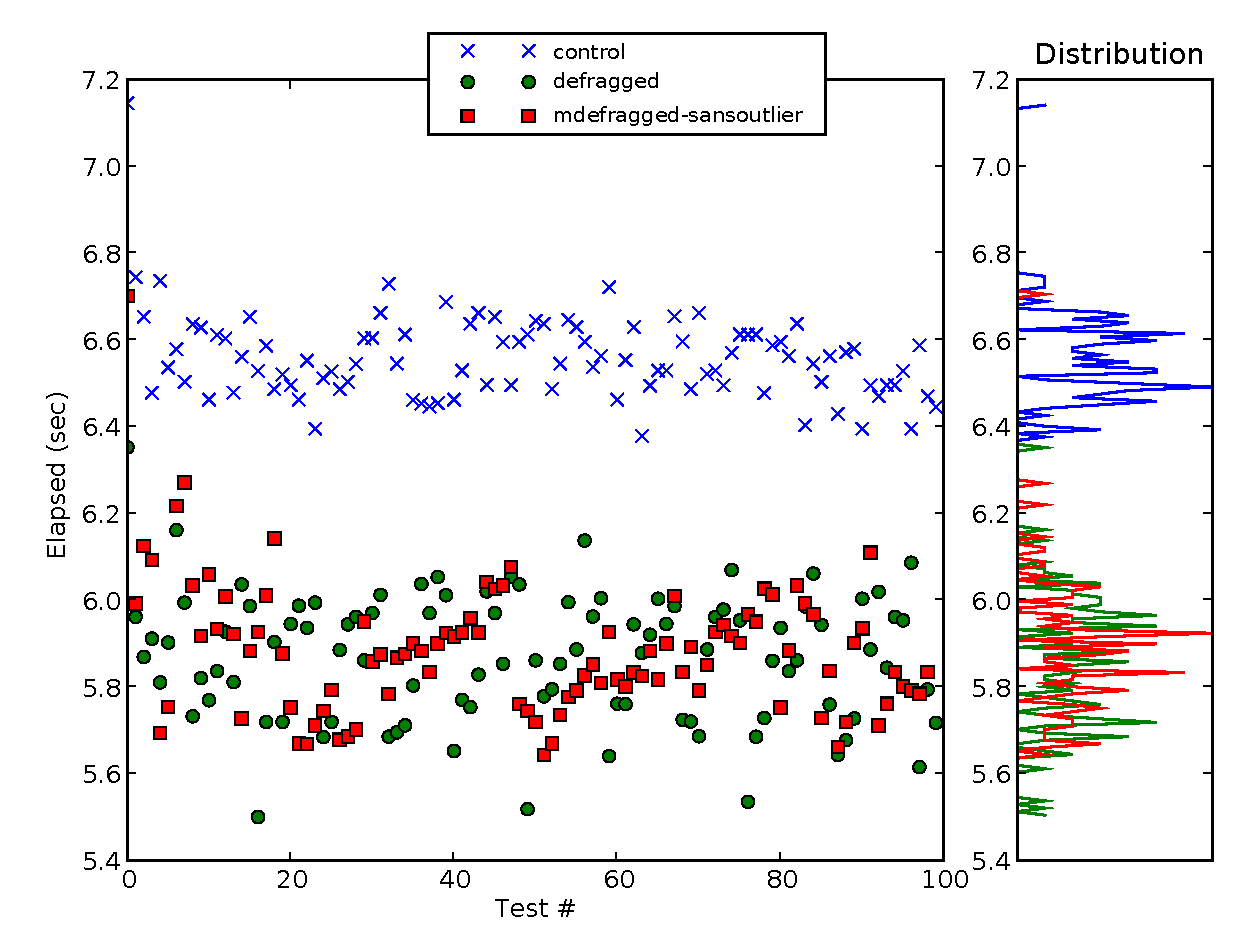
\includegraphics[scale=0.75]{mysql-chart.eps}
\caption{Startup times for MySQL}
\label{mysqlchart}
\end{figure*}

\section{Data Collected for MySQL Startup}

As noted in section \ref{sec:results}, server applications such as MySQL are easy to measure because it is easy to define the point at which they have ``started up'': when they are able to serve client requests.

For measurement purposes, a sample database containing two related MyISAM tables with various column types and indexes was defined. These tables were filled with 20,000 and 10,000 lines of pseudo-random data respectively. Although this data was randomly generated, it was only generated once; that is, although the data was arbitrary, both the control and experimental tests were operating on the \emph{same} arbitrary data.

The timing process, for each sample, took a beginning timestamp, called the init.d script for MySQL, and waited for it to return. Then, it connected to the server using the Python \texttt{MySQLdb} client module, and supplied it with a complex query involving data within and indexes on both tables. The query was limited to 10 rows, and once the
server supplied those rows to the client, the ending timestamp was taken. The results from 100 such timing runs are shown in Figure \ref{mysqlchart}.

The mean time elapsed between beginning and ending timestamps for the control was 6558.43 ms, with a standard deviation of 99.82 ms. After defragmentation with \texttt{defragment.py}, the mean time elapsed decreased by nearly a second to 5873.32 ms, with a standard deviation of 147.24 ms. The results after defragmentation with \texttt{mdefragment.py} were very similar, with a mean of 5884.01 ms and a standard deviation of 152.76 ms, after the removal of one outlier (8237 ms) from the result set.

Thus, both types of defragmentation resulted in a statistically significant change in the mean startup time of MySQL, a reduction of about a full second. The optimiziation, however, also increased the variance between samples significantly.

\begin{figure*}[!htb]
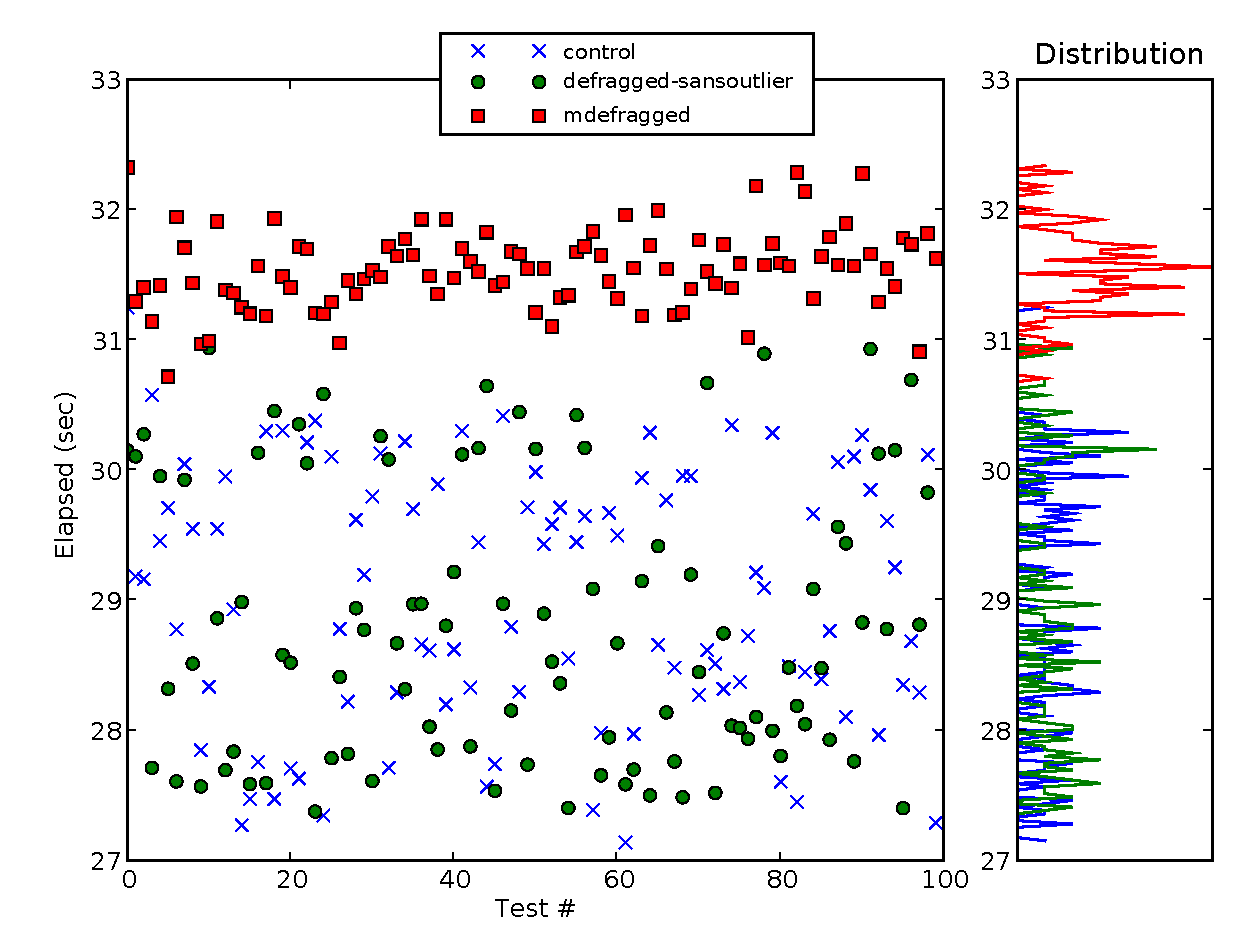
\includegraphics[scale=0.75]{kde4-chart.eps}
\caption{Startup times for X and KDE4}
\label{kde4chart}
\end{figure*}

\section{Data Collected for X \& KDE Startup}

The situation for testing KDE is even more complicated, since desktop environments like KDE are designed
to perform a wide range of disparate tasks. Such systems have not really started up \emph{entirely} until they are capable of performing every one of their varied functions. For example, it would not be enough to say that KDE has fully loaded when it is, say, possible to use its main menu to launch applications, because at that time KDE might still be busy loading other components, such as the background image manager, or the taskbar, or
the file management layer. It would be impractical to test each of these tasks individually in some way,
as we did with OpenOffice, so another method for finding the startup point must be used.

tests/kde4/results/kde4-times-control (100 lines):  Mean=29022.81  StdDev=972.04
tests/kde4/results/kde4-times-control-frecord (100 lines):  Mean=29833.02  StdDev=836.68
tests/kde4/results/kde4-times-defragged (100 lines):  Mean=29000.14  StdDev=2011.59
tests/kde4/results/kde4-times-defragged-sansoutlier (99 lines):  Mean=28827.84  StdDev=1057.64
tests/kde4/results/kde4-times-mdefragged (100 lines):  Mean=31543.05  StdDev=300.57
Outlier in defragged: 46058

\begin{figure*}[!htb]
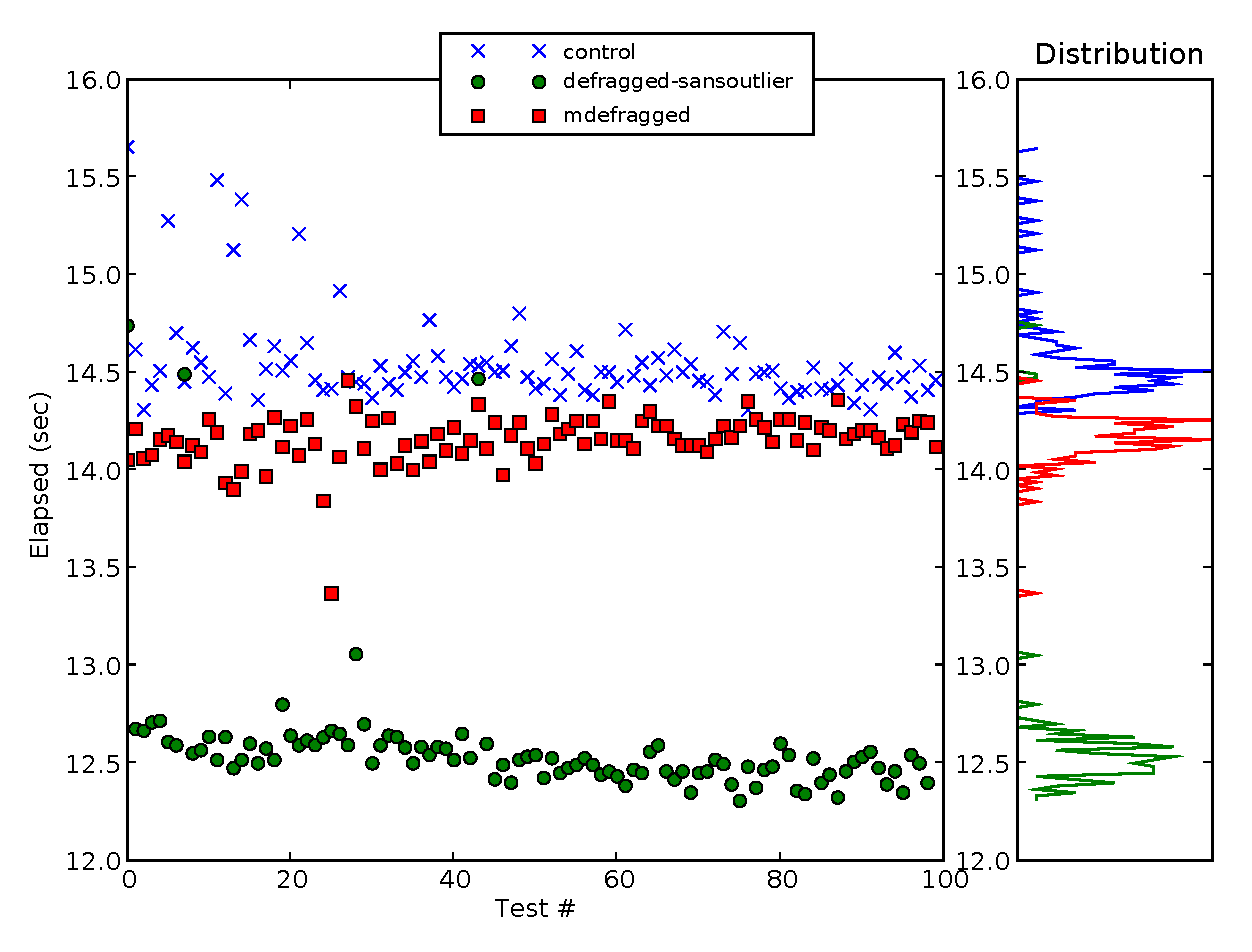
\includegraphics[scale=0.75]{openoffice-chart.eps}
\caption{Startup times for OpenOffice}
\label{oochart}
\end{figure*}

\section{Data Collected for OpenOffice Startup}

tests/openoffice/results/openoffice-times-control (100 lines):  Mean=14551.48  StdDev=232.81
tests/openoffice/results/openoffice-times-control-frecord (100 lines):  Mean=14797.68  StdDev=148.20
tests/openoffice/results/openoffice-times-defragged (100 lines):  Mean=12780.42  StdDev=1954.91
tests/openoffice/results/openoffice-times-defragged-sansoutlier (99 lines):  Mean=12587.40  StdDev=367.09
tests/openoffice/results/openoffice-times-mdefragged (100 lines):  Mean=14157.44  StdDev=128.04
Outlier in defragged: 31889

\section{Analysis of Results}

\section{Possible Future Work}\label{sec:future}

FIXME PARAGRAPH DUMP

For example, many hard disks, upon discovering that a particular block has gone bad, will silently
remap that block to some other place on disk\cite{remapping}. This is a good thing for ensuring
data integrity, but it makes Bolero's optimization strategy more difficult, because
its idea of the ``physical'' disk location is actually still a level of abstraction away from
the actual disk. To overcome this, the observer can compare its recorded response
times with expected times, based on an understanding of how disks typically work.
If the delay in going from one seemingly ``contiguous'' block to the next
is unexpectedly long, then we may be able to assume that one of the blocks involved
has been silently remapped to some distant part of the disk. Such blocks can then be
assumed by the reorganizer to have poor contiguity regardless of proximity to other
blocks.

A significant property of both Bolero reorganizers is that \emph{only data blocks} are moved; inodes are
unaltered by the process. This is because the \texttt{pyext2} library included with Bolero is not capable of moving inodes. This is the most significant remaining theoretical problem with the project. A given file's inode entry must be read first to locate its data blocks. Therefore, depending upon how scattered the inodes are on disk and in what order they must be read, they are almost certainly a significant remaining source of optimizable disk delays and seeks.

Concurrency presents another possible measurement hurdle. As mentioned above, the applications for
which startup time would benefit the most from Bolero are those applications which involve a
large number of pieces, all potentially scattered around the filesystem. However, there is no guarantee
that these pieces will always be loaded in the same order by the application. KDE, for example, might reasonably start its window manager and its taskbar at the same time. Because of a certain amount of random
variation in the computer's state before and during the loading process, this might result in
slightly different disk access patterns for the same application. During one run, the taskbar might finish loading just before the window manager, while in another run, the opposite might be true. Multiple
measurements will be necessary to see how much the optimization helps despite this unpredictability.

One final issue that must be addressed for accurate measurement is the effect of caching. Both
the operating system and the drive itself will be, in light of the inherent slowness of hard drives,
doing a lot of caching. The operating system's cache can probably be manipulated directly; more
investigation into the Linux kernel will be required, but I suspect that clearing the software
cache may be as simple as unmounting and remounting the partition. The hard drive's internal cache
may be tricker to deal with, but one possible strategy might be to simply load several large chunks of
unused data from the drive, thereby filling the drive cache entirely or mostly (depending upon the mapping
and replacement schemes used) with garbage information that has nothing to do with the activities being tested.
The purpose of all of this cache-busting is to involve the actual hard drive as much as possible
in the tests, because Bolero's optimizations have to do with the physical limitations of hard drives. Although caching certainly helps programs to start up faster, it also interferes with my ability to test Bolero's actual effectiveness.

Bolero can't deal well with large filesystems.

\section{Conclusion}

Assuming that Bolero does end up being significantly useful, there are a number of directions that
the project could go in. A few of them are mentioned above: Bolero might be portable to other
operating systems or filesystems, or it might be possible to use it on more complicated multi-partition
or multi-disk setups. Additionally, there are probably other, more complex observation-based reorganization schemes
besides the two suggested above.

Before any of this is worth considering, though, the basic premise must first be tested. Can disk
blocks be reorganized based on observations of usage patterns to significantly improve performance?
There might be tremendous performance gains. Or, the unpredictability and complexity of modern
computers and applications may mean that careful organization of blocks in a seemingly helpful
sequence may really result in little to no perceivable benefit. The development of Bolero should conclusively
show which of these is the case.

FIXME NON-BREAKING LINES IN BIBLIOGRAPHY URLS ARE ANNOYING.

\bibliography{report}{}
\bibliographystyle{plain}

\end{document}
